%
%  -- INTRODUCCION --
%
\par Richard Lemarchand es un game designer prominente en la industria de videojuegos. Trabajó en franquicias populares, como Gex, Soul Reaver y Uncharted \cite{RichardLemarchandcom}. Además, es profesor en la Universidad de Southern California (USC) \cite{RichardLemarchandcom}. En 2021, publicó un libro llamado “A Playful Production Process” \cite{lemarchandPlayfulProductionProcess2021}, donde explora una metodología de desarrollo basada en su experiencia como game designer, productor y profesor. \todo{TODO: Expandir} 
\par Para Lemarchand, hay una fuerte conexión entre game design y producción. Es por esto que en su metodología toma conceptos de ambos campos. De forma similar a Ramadan y Widyani, utiliza el libro "Game Design Workshop" \cite{fullertonGameDesignWorkshop2008} como punto de partida.
%
\begin{figure}[H]
  \centering
  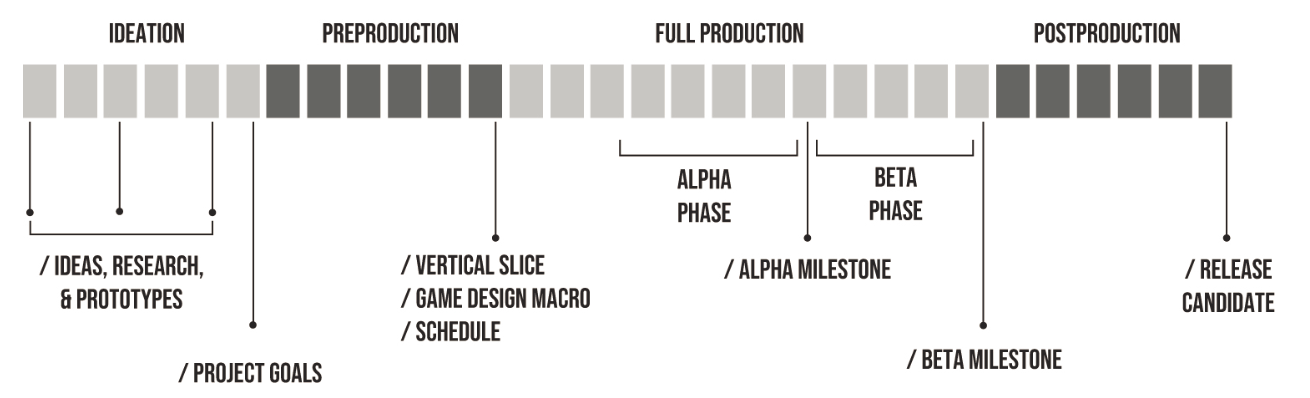
\includegraphics[scale=0.3]{image6.png}
  \caption{Etapas de la metodología propuesta por Lemarchand. Extraída de \cite{lemarchandPlayfulProductionProcess2021}.}
  \label{fig:x proceso de desarrollo Lemarchand}
\end{figure}
%
%
%  -- IDEATION --
%
\subsection{Ideation}
El proceso de desarrollo comienza en estae etapa, donde se definen una serie de objetivos llamados \textit{player experience goals}. Este concepto es propuesto por Fullerton, que los define como ``una serie de objetivos propuestos por el game designer, que indican el tipo de experiencia que los jugadores tendran durante el videojuego." \cite{fullertonGameDesignWorkshop2008} (Traducción propia).
\par Ejemplos de estos objetivos son ``los jugadores sentirán curiosidad por explorar un universo desconocido.'' o ``los jugadores colaborarán para sobrevivir un mundo post apocalíptico.''. Para establecer estos objetivos, Lemarchand propone una serie de herramientas:
\begin{itemize}
    \item Brainstorming: activadad grupal o individual donde se generan ideas espontaneamente. Lemarchand recomienda enfocarse en la cantidad de ideas, sin preocuparse por su calidad, resaltando la importancia de escribir todas las ideas, incluso las que parecen malas o irrelevantes.
    \item Mind mapping: esta técnica consiste en escribir una idea central y luego conectar ideas relacionadas. 
    \begin{figure}[H]
        \centering
        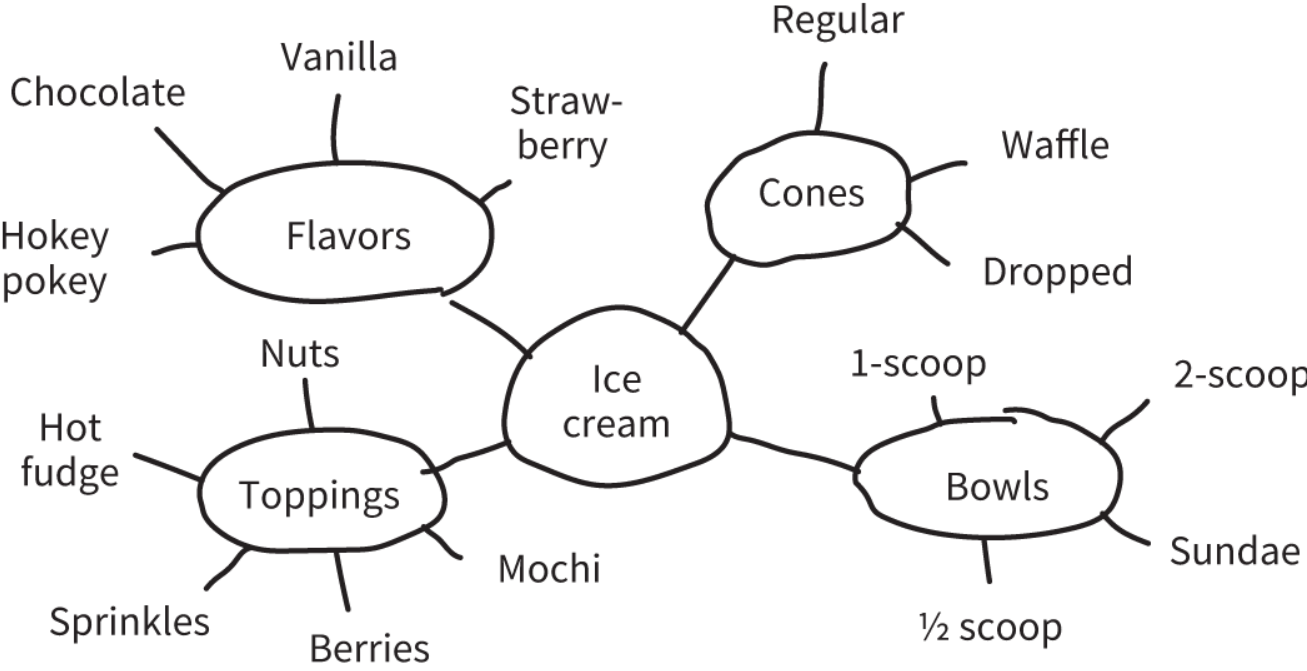
\includegraphics[scale=0.3]{mind_map.png}
        \caption{Ejemplo de un \textit{mind map}. Extraída de \cite{lemarchandPlayfulProductionProcess2021}.}
        \label{fig:x ejemplo de un mind map Lemarchand}
    \end{figure} 
    \item Automastim: este ejercicio consiste en configurar un temporizador y escribir sin parar durante un tiempo determinado. El objetivo es generar ideas espontaneamente, sin preocuparse por la calidad de las mismas.
\end{itemize}
%
%
\subsubsection{Prototipado}
\par Realizar prototipos es una parte fundamental de esta etapa. Lemarchand recomienda empezar con a prototipar lo antes posible, enfocandose en explorar distintas ideas. El objetivo de un prototipo es encontrar una un número pequeño de mecánicas (inclusive una sola) que sea interesante o divertida. 
\par Para ayudar en la creación de prototipos, Lemarchand define algunos conceptos de game design. Primero define una \textit{mecánica} como ``reglas y procesos en un juego que lo vuelven funcional e interactivo.''(Traducción propia) \cite{lemarchandPlayfulProductionProcess2021}. Las mecánicas crean acciones llamadas \textit{game verbs}. Algunos ejemplos son saltar, caminar o disparar. Finalmente, define \textit{player activity} como ``las formas en las que un jugador usa un game verb en particular'' (Traducción propia) \cite{lemarchandPlayfulProductionProcess2021}. Por ejemplo, un jugador puede usar la barra espaciadora para ejecutar el \textit{game verb} de saltar. O puede ser un concepto mas abstracto, como tratar de encontrar un final diferente en una historia interactiva. \textit{player activity} es ``el resultado de combinar mecánicas, game verbs y narrativa con las acciones del jugador'' (Traducción propia) \cite{lemarchandPlayfulProductionProcess2021}.
\par Estos conceptos son importante porque para Lemarchand, un prototipo debe explorar un \textit{player activity} en particular para decidir si es interesante o no. Para ello, propone una serie de preguntas que un prototipo debe responder:
\begin{itemize}
    \item ¿Qué \textit{player activity} estoy prototipando?
    \item ¿Qué \textit{game verbs} estoy explorando?
    \item ¿Qué emocion evoca este \textit{player activity}?
    \item Este prototipo, ¿contesta alguna pregunta de game design? \todo{TODO: reescribir}
\end{itemize}
\bigbreak
\par Similar a Anderson, Lemarchand propone realizar tanto prototipos físicos como digitales. Los prototipos físicos son más rápidos de hacer, pero limitan el tipo de mecánicas que se pueden explorar. Por otro lado, los prototipos digitales son más lentos de hacer, pero permiten explorar una mayor variedad de mecánicas.
\par Playtesting es una parte importante del proceso. Lemarchand recomienda entregar los prototipos a otras personas lo antes posible, y observar cómo interactuan con ellos.
%
%
\subsubsection{Project goals}
\par El objetivo final de la etapa de \textit{Ideation} es definir los \textit{project goals}. La idea es que establecer objetivos claros para el proyecto ayuda a guiar el proceso de desarrollo en las siguientes etapas. Lemarchand separa los \textit{project goals} en dos categorias, \textit{experience goals} y \textit{design goals}. 
\bigbreak
\par Segun Lemarchand, un \textit{experience goal} es ``el tipo de experiencia que se le quiere dar al jugador, generalmente explicada en términos de la experiencia emocional.'' (Traducción propia) \cite{lemarchandPlayfulProductionProcess2021}. Ejemplos de esto puede ser la satisfacción de ganar o el miedo al jugar un juego de terror. La figura \ref{fig:x ejemplo de experience goals Lemarchand} muestra los \textit{experience goals} establecidos para Uncharted, uno de los juegos en los que el escritor trabajó.
%
\begin{figure}[H]
    \centering
    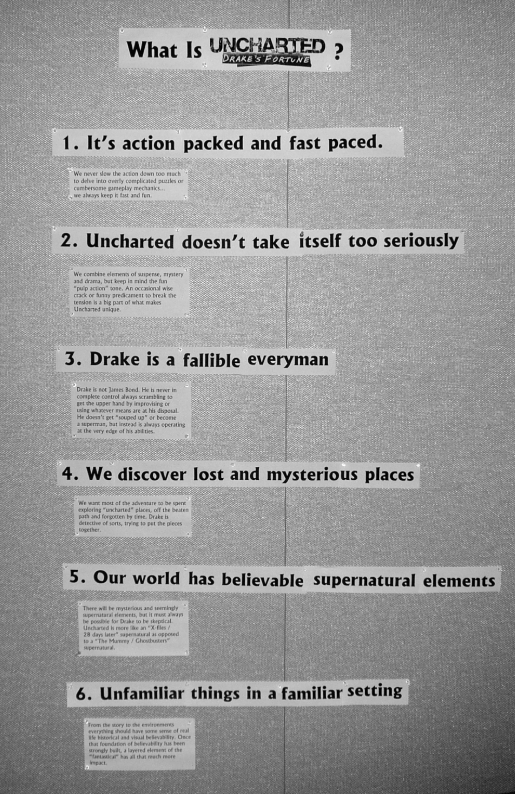
\includegraphics[scale=0.5]{experience_goals.png}
    \caption{``Experience goals'' del videojuego Uncharted. Extraída de \cite{lemarchandPlayfulProductionProcess2021}.}
    \label{fig:x ejemplo de experience goals Lemarchand}
\end{figure} 
%
\par Por otro lado, los \textit{design goals} son las mecánicas que complementan a los \textit{experience goals}. Algunas categorias comunes son:
\begin{itemize}
    \item La plataforma en la que se desarrollará el videojuego (PC, consola, móvil, etc.).
    \item Mecánicas, \textit{game verbs} y \textit{player activities}.
    \item El género del videojuego (plataforma, aventura, rol, etc.).
    \item La dirección artística del videojuego (estilo visual, música, etc.).
\end{itemize}
%
%
%  -- PRE PRODUCTION --
%
\subsection{Pre-production}
\par Lemarchand define a \textit{pre-production}(pre-producción en español) como la etapa donde se se establece el \textit{game design} y el plan a seguir durante la etapa de \textit{prorduction}. Al final de esta etapa, se obtienen 3 artefactos: un \textit{vertical slice}, un \textit{game design macro} y un \textit{schedule} \cite{lemarchandPlayfulProductionProcess2021}.
%
%
\subsubsection{Vertical Slice}
Un \textit{vertical slice} es una demo de alta calidad de un videojuego \cite{lemarchandPlayfulProductionProcess2021}. Tanto gráficos, sonido, mecánicas y narrativa deben estar lo suficientemente pulidos como para ser considerados parte del producto final. 
\par Esta demo se construye iterativamente a partir de intentos anteriores, siguiendo un \hyperref[sec:modelos_evolutivos]{modelo evolutivo}. Para ello, se define una mecánica, se crea un prototipo para probarla, se realiza \textit{playtesting} y se evalúa el resultado. Al final de cada iteración se revisa si el prototipo cumple con los \textit{experience goals} definidos, y si es necesario, se realizan cambios. Este proceso se repite hasta que se obtiene un \textit{vertical slice} que cumple con los objetivos del proyecto.
\begin{figure}[h]
    \centering
    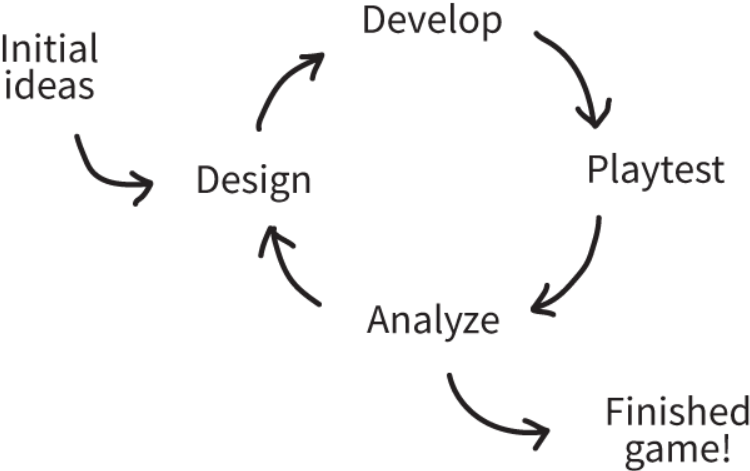
\includegraphics[scale=0.5]{vertical_slice_iteration.png}
    \caption{Proceso iterativo para la creación de un \textit{vertical slice}. Extraída de \cite{lemarchandPlayfulProductionProcess2021}.}
    \label{fig:x iteracion vertical slice}
\end{figure} 
